The MMB 3.1 can be downloaded from \url{macromodelbase.com/download}. The version for windows is \texttt{mmb-electron-win.exe}, for macOS it is \texttt{mmb-electron-mac.dmg}, and for Linux directly download the source code from the release on github at
\url{https://github.com/IMFS-MMB/mmb-gui-electron/tags}.\footnote{Linux users will have to build from source using \texttt{npm}. Find more info on our github page.}
The Windows version and the Mac version of the file autoinstall the MMB on your computer and opens the redesigned frontend of the MMB. 

The files for carrying out the simulations of the models are written in MATLAB, so either some version of MATLAB or a recent version of its freeware clone, OCTAVE, must be installed on your computer. In the case of Matlab, one also needs the \textit{Optimization Toolbox} as well as the \textit{Statistics Toolbox} in order to be able to run all models in the Modelbase.\footnote{For the time being there are some models, which cannot be simulated with Octave. The list of models contains: NK\_ET14, NK\_FLMF18, NK\_GK11, US\_AJ16, US\_CMR14, US\_CMR14noFa, US\_FRB08, US\_FRB08mx, US\_IR15, EA\_Q14. The problems with the latter model exist only with Octave 4.4.0.}
For model solution the program utilizes DYNARE, which can be downloaded free of charge from the web.\footnote{\url{http://www.dynare.org}} Under Windows, double-clicking on the downloaded DYNARE exe-file opens a set of steps that guide you through the installation. Under macOS, locate the downloaded pkg-file in Finder, and Control-click the icon to select Open from the menu, thus creating an exception for the app to be installed. The installer will then guide you through the installation. To install Linux verison of Dynare please follow the instructions on the Dynare Wiki\footnote{The DYNARE Wiki install guide for Ubuntu and Debian can be found at \url{http://www.dynare.org/DynareWiki/InstallOnDebianOrUbuntu}}.

\subsection*{Compatibility}

REVISE THIS SECTION

We have tested the MMB 3.0 with DYNARE 4.5.6 and 4.5.7. Earlier versions may work but have not been tested.\\
On Windows, DYNARE 4.5.6 is compatible with OCTAVE 4.4.0, whereas DYNARE 4.5.7 is compatible with OCTAVE 4.4.1. Both Dynare versions are compatible with  MATLAB R2007b and later. For macOS, the compatibility between DYNARE and MATLAB is the same. However, at the time of this release, the highest OCTAVE-supported version of DYNARE is 4.5.6 (compatible with OCTAVE 4.4.0 on macOS).\\


\subsection*{Further steps before running comparisons}
When using MATLAB, one has to add the DYNARE path to MATLAB. In order to do so, open MATLAB and choose \textit{Set path} from the \textit{File} menu. Use the option \textit{Add folder} and browse to the directory where you have installed DYNARE. The DYNARE subfolder that has to be added is called \textit{MATLAB}.

%Before running simulations with the MMB, you need to specify whether you want to run the simulations in MATLAB or OCTAVE. In order to do so, click on settings on the upper-right corner of the MMB as shown in the Figure 'Settings'. 
Before running simulations with the MMB, you need to specify whether you want to run the simulations in MATLAB or OCTAVE. In order to do so, click on `Menu' on the upper-right corner of the MMB and then on `Settings', as shown in the Figure 'Settings'. It opens a window, in which you have the option either to let the program scan for versions of MATLAB and OCTAVE installed on your computer, or to search manually. If the scan finds more than one version of MATLAB or OCTAVE, you can choose from the list of programs in this subwindow by clicking on the small arrows on the right side. Note that the scan only looks in common directories as scanning the whole system would take too long. If the scan does not find the desired installation, click on `Find manually', select whether you want to add MATLAB or OCTAVE to the list of executables  and browse to the folder of the installation. Select the executable file which opens the program and click on `Open'. If you want to remove an entry from the selection menu, select it and click on `Remove selected'.

You can follow the same steps  to select or delete a version of DYNARE on which you want to run the simulations.

Finally, the `Settings' menu also allows you to set a path of the MMB. You can either select a folder by clicking directly into the path field and extract the files shipped with the MMB into this folder by clicking on `Extract files'. You can also click on `Select folder' to choose a folder in which you already have installed the MMB. This option can be used if you have installed more than on version of the MMB, e.g. an original one and one in which you changed  or added models or policy rules. Thirdly, you can click on `Use builtin' to reset the folder and use the default MMB files shipped with user interface you are using.

To check whether your installations of MATLAB/OCTAVE and DYNARE are compatible with the MMB, click on `Check compatibility' in the lower left corner. This check can take up to 30 seconds. 

You can close the `Settings' window by clicking on `Close' in the lower right corner or on the cross in the upper right corner.

\begin{figure}[H]%[htb]
\centering
\caption{\textsc{Settings}}
\vspace{0.2cm}
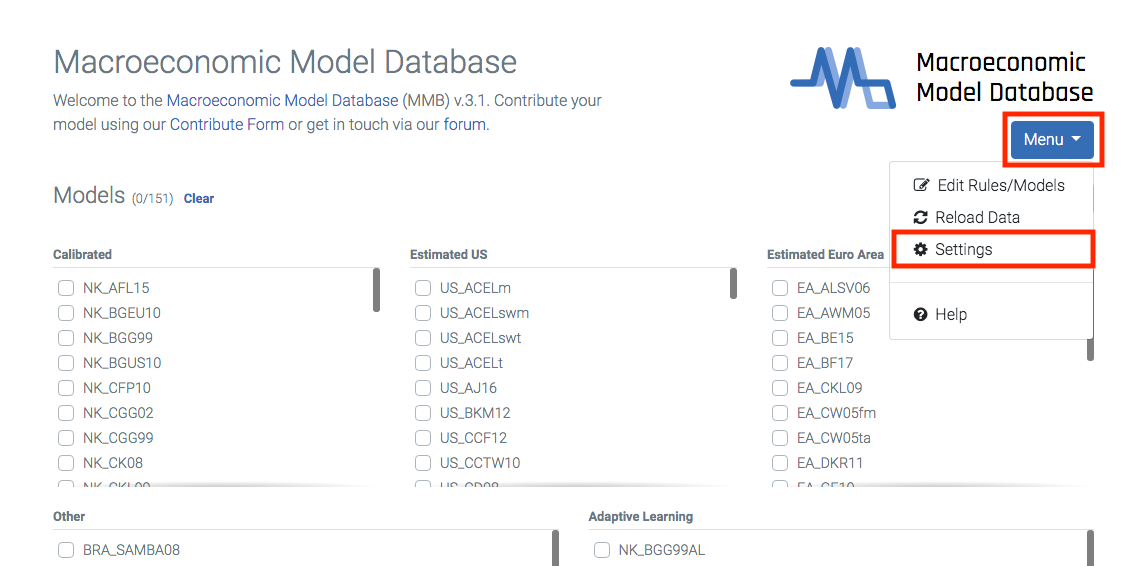
\includegraphics[width=12cm,keepaspectratio]{settings31}\\[1cm]
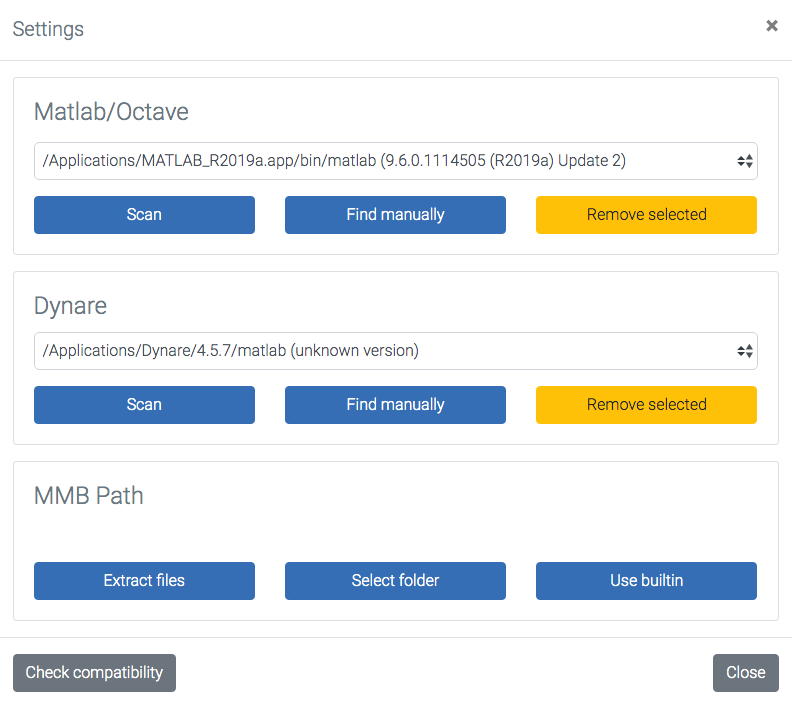
\includegraphics[width=9cm,keepaspectratio]{settings2_31.png}
\label{img:Settings}
\end{figure}






